\chapter{Related Work}\label{cap:relatedwork}
\section{Related writings}
\subsection*{Deeper Learning With QR Codes and Augmented Reality: A Scannable Solution for Your Classroom}

In the realm of education, the integration of technology has revolutionized teaching and learning processes.  Drawing inspiration from Monica Burns' book "Deeper Learning With QR Codes and Augmented Reality: A Scannable Solution for Your Classroom", exploring how \ac{AR} and \ac{QR} codes can enhance learning experiences and engage students in interactive educational content.

\acf{AR} offers a unique opportunity to create immersive and interactive learning environments. By overlaying digital content onto real-world objects, \ac{AR} provides students with an interactive tool for learning. As Monica Burns highlights, \ac{AR} can be likened to a "window to interactive learning" \cite{Burns2016}. Students can unlock a wealth of three-dimensional models, virtual objects, and multimedia resources through \acf{QR} codes. By scanning these \ac{QR} codes using smartphones or tablets, students' surroundings are enhanced with digital content.

Educators worldwide have embraced \ac{AR} as a powerful tool for instructional design. Teachers can seamlessly integrate \ac{AR} into their lessons by leveraging \ac{AR} apps and printing corresponding trigger images. For instance, using an \acf{AR}, students can explore the intricacies of the human body by scanning large posters of anatomical models. As Burns emphasizes, using \ac{AR} captivates students' attention and provides a unique opportunity to interact with and deepen their understanding of content \cite{Burns2016}.

Unleashing digital resources alongside \ac{AR}, \ac{QR} codes has become an efficient way to connect physical and digital resources. By scanning these codes using mobile devices, students gain instant access to a wealth of online content. With a simple scan, \ac{QR} codes can link students to websites, videos, interactive quizzes, and other digital resources, expanding their learning beyond the confines of traditional materials.

\ac{QR} codes have become a versatile tool in the classroom, empowering teachers to deliver digital content seamlessly. Educators can create \ac{QR} codes to supplement lessons, provide additional resources, or foster independent research. Students can embark on self-directed learning journeys by incorporating \ac{QR} codes into lesson plans, exploring personalized content, and engaging in collaborative projects. The ease of use and immediate access to digital resources make \ac{QR} codes invaluable in modern classrooms.

Integrating \ac{AR} and \ac{QR} codes in education holds tremendous potential for transforming learning experiences. Educators can foster engagement, deepen understanding, and inspire lifelong learners by immersing students in interactive virtual worlds and providing access to vast digital resources. As we embrace Monica Burns' notion of "tasks before apps," we must approach these technologies with clear pedagogical objectives \cite{Burns2016}. By strategically integrating \ac{AR} and \ac{QR} codes, we can create meaningful and impactful learning experiences that prepare students for success in a technology-driven world.


\section{Related apps}
\subsection*{Snapchat}
Regarding \ac{AR} applications, Snapchat \cite{Snapchat} stands out as a platform that pioneers the use of \ac{AR} and revolutionises how we create, explore, and play with digital content. Harnessing the power of their \ac{AR} module and Snap \ac{AR} \cite{SnapAR} enables users worldwide to scan their surroundings and discover valuable information. With just a tap on the Camera screen, the \ac{AR} Bar unfolds.

\begin{wrapfigure}{r}{0.4\textwidth}
    \centering
    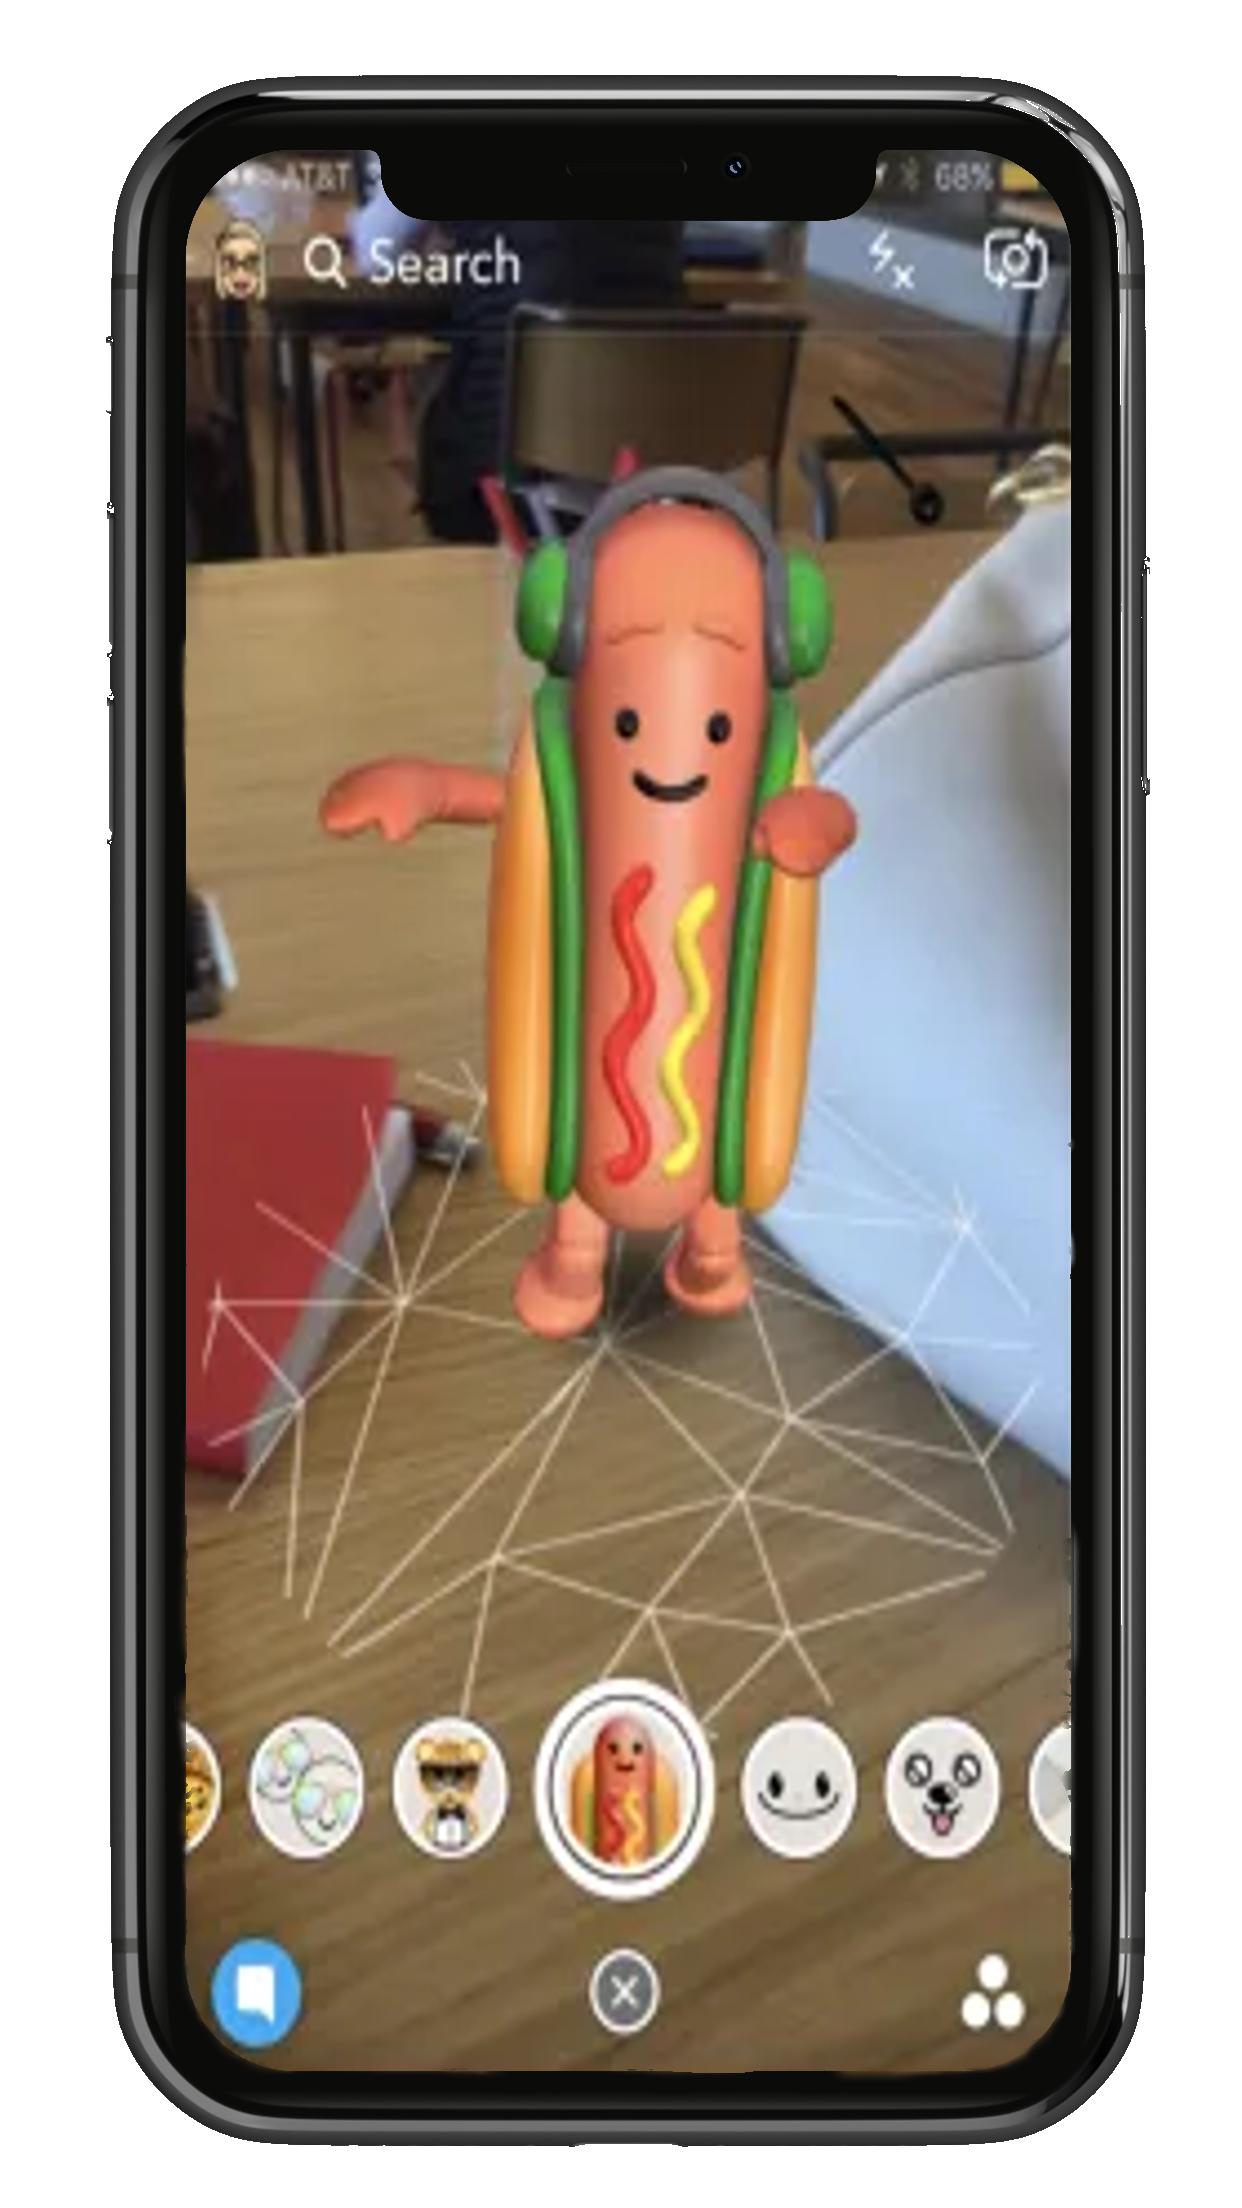
\includegraphics[width=0.32\textwidth]{img/related-apps/Snapchat.png}
    \caption{Snapchat AR}
    \label{fig:snapchat}
\end{wrapfigure}

What sets Snapchat \ac{AR} apart is its commitment to accessibility. The introduction of the Web Lens Builder and Lens Studio tools has democratised the creation of \ac{AR} Lenses, making it easier for aspiring creators to bring their visions to life. Moreover, Snapchat has embraced the incorporation of real-world physics and real-time data integrations, elevating the realism and immersion of their \ac{AR} experiences to new heights.

Snapchat AR brings a fantastic array of special Lenses, each presenting a unique and captivating visual journey. With a plethora of playful animations and informative overlays, the creative possibilities are boundless. Moreover, it boasts a diverse collection of filters designed to enhance the user's appearance or transport them into an array of different characters. What's more, these filters are regularly updated, guaranteeing users a constant stream of exciting options.

However, it's important to acknowledge that Snapchat AR does have its limitations. A consistent internet connection is imperative to browse for new lenses and filters, which may prove challenging in certain circumstances. Additionally, while Snapchat \ac{AR} offers a compelling experience, it needs to improve in terms of functionality when compared to more specialised \ac{AR} applications.



\subsection*{Pokemon Go}
In mobile gaming, Pokemon Go has become a global sensation by leveraging the power of \ac{AR}. The game's \ac{AR}+\cite{AR+} mode takes the concept of \ac{AR} to new heights by seamlessly merging the Pokemon universe with the player's real-world surroundings. Through this innovative approach, Pokemon come alive and appear anchored to the user's environment, providing exciting opportunities for an interactive gameplay experience.


\begin{wrapfigure}{r}{0.4\textwidth}
    \centering
    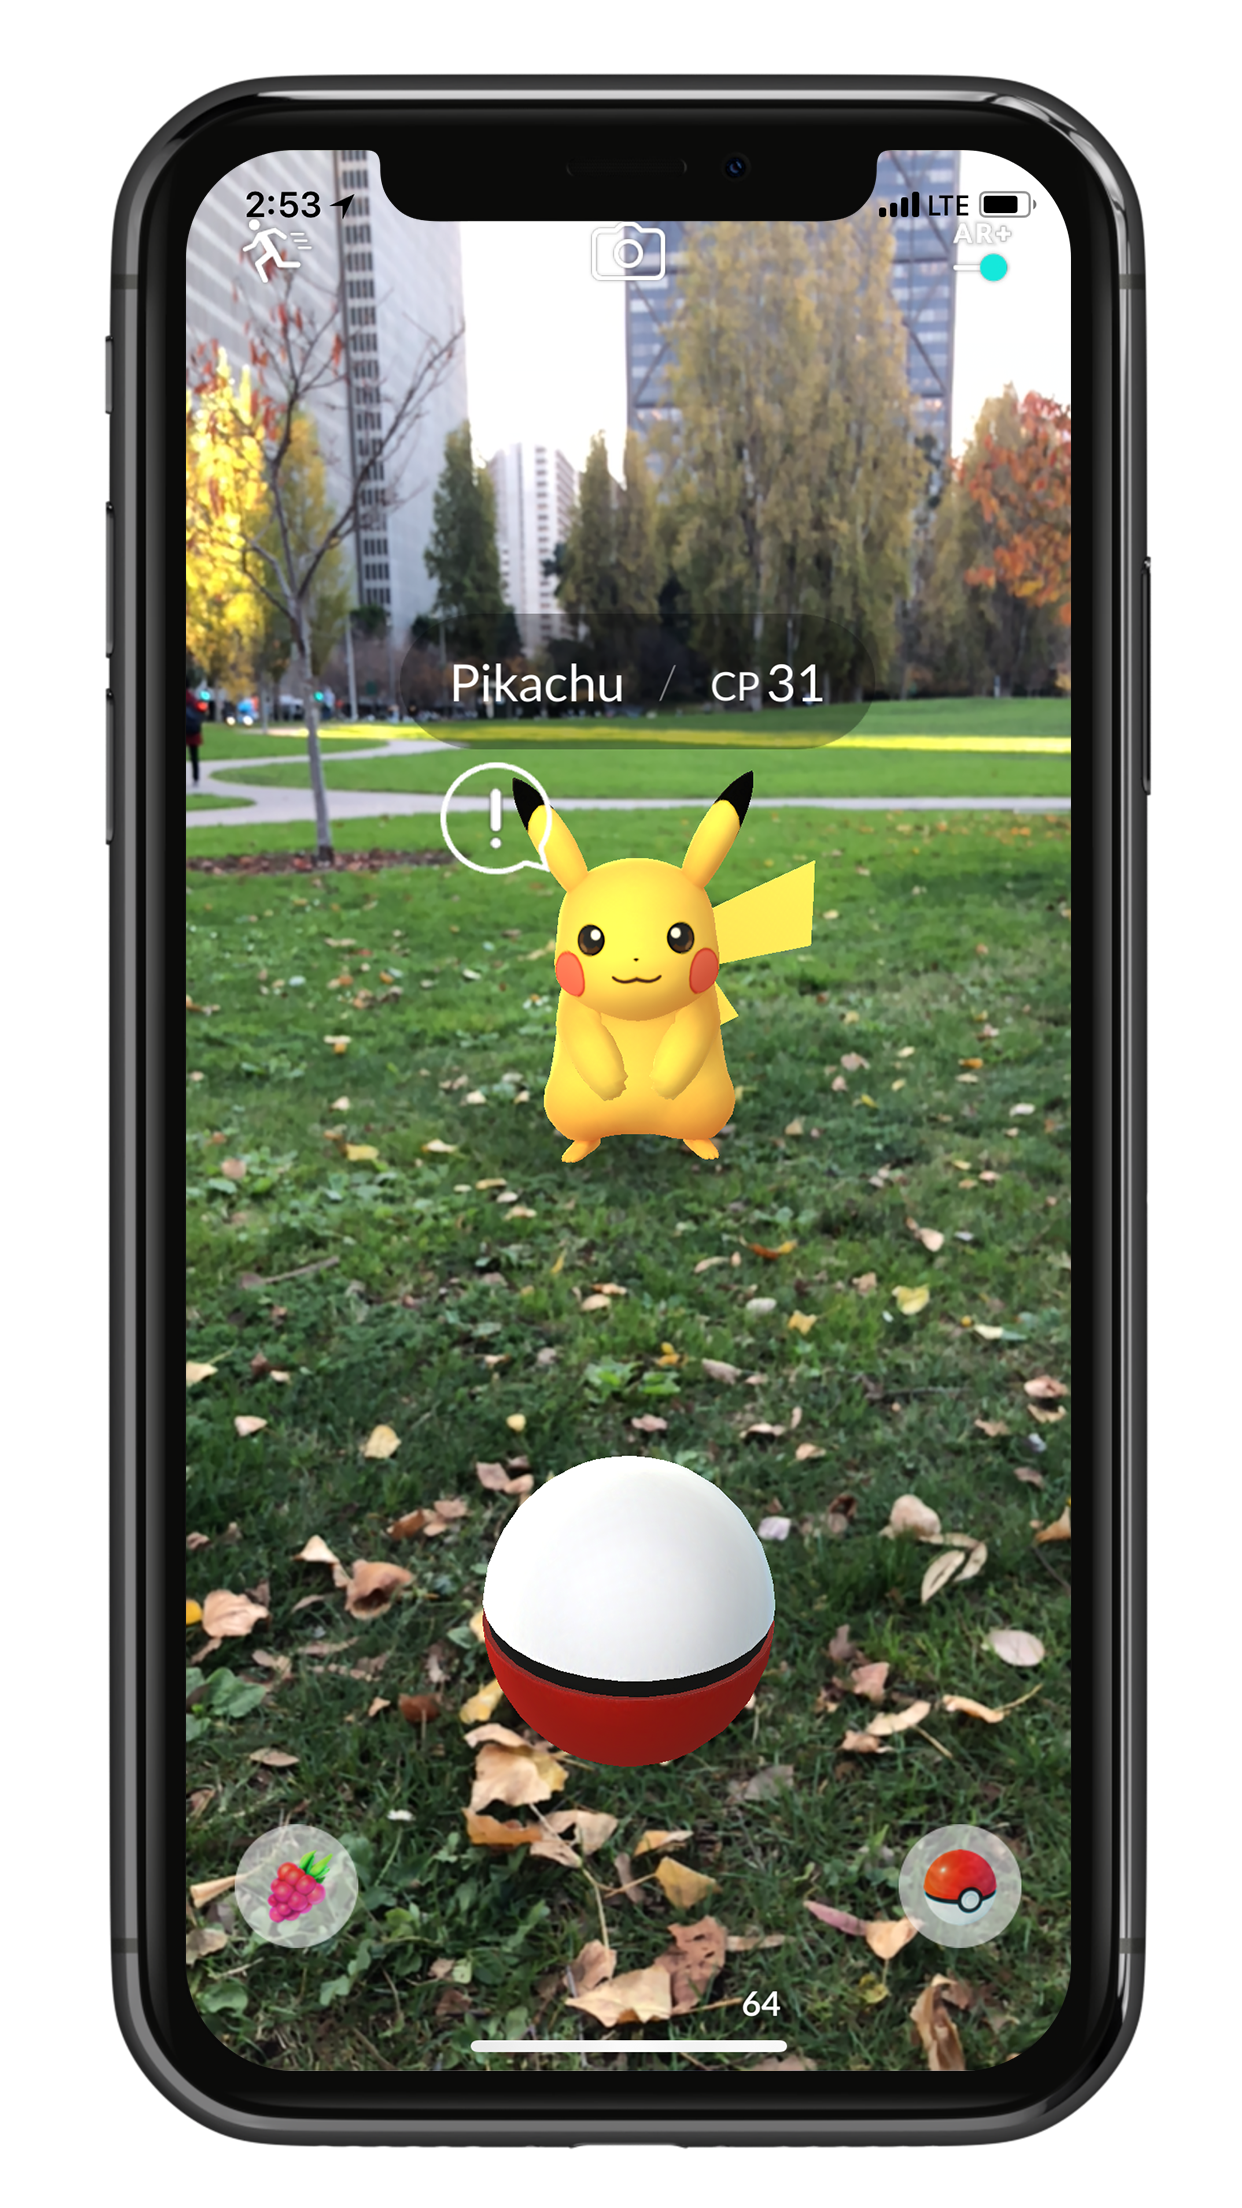
\includegraphics[width=0.4\textwidth]{img/related-apps/PokemonGO.png}
    \caption{PokemonGO}
    \label{fig:PokemonGO}
\end{wrapfigure}

In \ac{AR}+ mode, Pokemon Go brings an added layer of realism to the gameplay experience. Players can approach, walk toward, or even move around these digital creatures by fixing Pokemon to specific points in the real world, as shown in Figure \ref*{fig:PokemonGO}. The Pokemon in \ac{AR}+ mode possess an uncanny awareness of the player's proximity and movement, requiring strategic and cautious approaches to maximise successful encounters.

In contrast, the \ac{AR} mode in Pokemon Go detaches Pokemon from the real-world environment, lacking the anchor points and awareness of the player's location and movement found in AR+ mode.
The enhanced \ac{AR} features in Pokemon offer players a captivating and dynamic experience. As they explore their surroundings, Pokemon seemingly inhabit their world, creating magical moments for excellent throws and captivating photos. The fusion of \ac{AR} with the beloved Pokemon franchise has captivated millions of players worldwide.

Like Snapchat AR, Pokemon Go relies on a consistent internet connection to enable the \ac{AR} features. This requirement may pose challenges in situations where a stable connection is unavailable. Additionally, the GPS needs to be enabled to play Pokemon Go, which may drain the battery life of mobile devices. Despite these limitations, Pokemon Go has become a global phenomenon, demonstrating the power of \ac{AR} in mobile gaming.